\section{Розв'язок}

\subsection{Дискретизація простору параметрів}

Дискретизуємо простір параметрів $X$.
Введемо невелике $\delta x$ таке,
щоб ймовірність того, що значення потрапляє в рамки гіперкубу
$\left[ x - \frac{\delta x}{2}; x + \frac{\delta x}{2} \right]$,
приблизно дорівнювала добутку щільності розподілу в його центрі
на його об'єм
\begin{equation*}
  \mathbb{P}\left( \xi \in \left[ x - \frac{\delta x}{2};
                                  x + \frac{\delta x}{2} \right] \right)
  \approx p\left( x \right) \cdot \delta x^n,
\end{equation*}
де
\begin{equation*}
  \left( x \pm \frac{\delta x}{2} \right)_i = x_i \pm \frac{\delta x}{2},\qquad
  i = 1..n.
\end{equation*}
Далі треба розбити простір на гіперкуби
зі стороною $\delta x$ і вважати,
що коли величина потрапляє на територію певного гіперкубу,
то вона дорівнює значенню в його центрі.

Відомо, що параметри $x$ --- набори коефіцієнтів нормованих головних компонент,
тобто мають стандартний гаусовий розподіл.
Ймовірність того, що було згенеровано саме такий набір
\begin{equation*}
  \mathbb{P}_X\left( x \right)
  = \delta x^n \cdot \prod_{i=1}^n
    \frac{\exp{\left( - \frac{x_i^2}{2} \right)}}{\sqrt{2 \cdot \pi}}.
\end{equation*}

Введемо зручне позначення для шуму в пікселі $i$
\begin{equation*}
  y_i = t_i - f_i\left( x \right).
\end{equation*}
Розглядається одне зображення $t$.
З контексту буде зрозуміло, яке значення має $x$.
Ймовірність того, що обличчя на даному зображенні отримано з параметрами $x$
\begin{equation*}
  \mathbb{P}_Y\left( t \;\middle|\; x \right)
  = \delta x^{w \cdot h} \cdot \prod_{i \in I}
    \frac{\exp{\left\{- \frac{y_i^2}
           {2 \cdot \sigma^2_t} \right\}}}
           {\sqrt{2 \cdot \pi \cdot \sigma^2_t}}.
\end{equation*}

Відхилення проекції опорної точки $l$ моделі,
отриманої з параметрами $x$,
від реального положення опорної точки на зображенні,
позначимо $\Delta_l$
\begin{equation*}
  \Delta_l\left( x \right)
  = P^2_{\theta_M}\left( G_l\left( x \right) \right) - \theta_l,
  \qquad l \in L.
\end{equation*}
Ймовірність того, що параметри $x$ приймають саме такі значення,
якщо відомі координати опорних точок,
\begin{equation*}
  \mathbb{P}_L\left( x \right)
  = \delta x^{\left| L \right|} \cdot \prod_{l \in L}
      \frac{\exp{\left\{- \frac{\Delta_l^2\left( x \right)}
           {2 \cdot \sigma^2_L} \right\}}}
           {\sqrt{2 \cdot \pi \cdot \sigma^2_L}}.
\end{equation*}

Сумісна ймовірність зображення $t$ та параметрів $x$
\begin{equation*}
  \mathbb{P}\left( x, t \right)
  = \mathbb{P}_Y\left( t \;\middle|\; x \right)
    \cdot \mathbb{P}_X\left( x \right)
    \cdot \mathbb{P}_L\left( x \right)
\end{equation*}

\subsection{Інтервальна функція витрат}

Розглянемо функцію витрат,
за якої вірним є будь-який набір параметрів,
що знаходиться в $\delta$-околі дійсного набору $x$,
а за всі інші сплачується штраф $1$.

Для максимізації розглянемо логарифми ймовірностей,
тому що це зручніше,
ніж максимізація добутку кількох десятків тисяч або мільйонів значень
\begin{equation*}
  \begin{split}
    \mathbb{P}_X\left( x \right)
    &= \ln{\delta x^n} +
        \sum_{i = 1}^n
        \left\{
          - \frac{x_i^2}{2}
          - \frac{\ln{2} + \ln{\pi}}{2}
        \right\}, \\
    \mathbb{P}_Y\left( t \;\middle|\; x \right)
    &= \ln{\delta x^{w \cdot h}} +
        \sum_{i \in I}
        \left\{
          - \frac{y_i^2}{2 \cdot \sigma^2}
          - \frac{\ln{2} + \ln{\pi} + \ln{\sigma^2}}{2}
        \right\}, \\
    \mathbb{P}_L\left( x \right)
    &= \ln{\delta x^{\left| L \right|}} +
        \sum_{l \in L}
        \left\{
          - \frac{\Delta_l^2\left( x \right)}{2 \cdot \sigma_L^2}
          - \frac{\ln{2} + \ln{\pi} + \ln{\sigma_L^2}}{2}
        \right\}.
  \end{split}
\end{equation*}
Приберемо константні доданки,
що не впливають на результат максимізації ймовірності
появи даного зображення $t$ з даними параметрами $x$
\begin{equation*}
  \sum_{i \in I}
    \left\{
      - \frac{y_i^2}{2 \cdot \sigma^2}
      - \frac{\ln{\sigma^2}}{2}
    \right\}
  +
  \sum_{l \in L}
    \left\{
      - \frac{\Delta_l^2\left( x \right)}{2 \cdot \sigma_L^2}
      - \frac{\ln{\sigma_L^2}}{2}
    \right\}
  - \sum_{i = 1}^n \frac{x_i^2}{2}
  \to \max\limits_{x \in X}.
\end{equation*}
Помножимо на $-2$ та винесемо логарифм дисперсії за знак суми
\begin{equation}\label{eq:minimize}
  \left| I \right| \cdot \ln{\sigma^2}
  + \left| L \right| \cdot \ln{\sigma_L^2}
  + \sum_{i \in I} \frac{y_i^2}{\sigma^2}
  + \sum_{l \in L} \frac{\Delta_l^2\left( x \right)}{\sigma_L^2}
  + \sum_{i = 1}^n x_i^2
  \to \min\limits_{x \in X}.
\end{equation}
Замінимо дисперсію її оцінкою
\cite{BorovkovMS}
\begin{equation*}
  \left| I \right|
  \cdot \ln{
    \frac{\sum\limits_{i \in I} y_i^2}
         {\left| I \right| - 1}}
  + \left| I \right| - 1
  + \left| L \right|
  \cdot \ln{
    \frac{\sum\limits_{l \in L} \Delta_l^2\left( x \right)}
         {\left| L \right| - 1}}
  + \left| L \right| - 1
  + \sum_{i = 1}^n x_i^2
  \to \min\limits_{x \in X}.
\end{equation*}
Позбавимося константних доданків
\begin{equation*}
  \left| I \right|
  \cdot \ln{
    \frac{\sum\limits_{i \in I} y_i^2}
         {\left| I \right| - 1}}
  + \left| L \right|
  \cdot \ln{
    \frac{\sum\limits_{l \in L} \Delta_l^2\left( x \right)}
         {\left| L \right| - 1}}
  + \sum_{i = 1}^n x_i^2
  \to \min\limits_{x \in X}.
\end{equation*}
В загальному випадку зображення містить не тільки обличчя.
Генерація усіх можливих фонів для кожної моделі є недоцільною.
Потрібно отримати формулу,
яка не прив'язана до кожного пікселя вхідного зображення $t$.
Для цього перепишемо доданки як середньоквадратичні відхилення
\begin{equation*}
  \left| I \right|
  \cdot \ln{\widetilde{y}^2}
  + \left| L \right|
  \cdot \ln{\left[ \widetilde{\Delta}^2\left( x \right) \right]}
  + \left( n - 1 \right) \cdot \widetilde{x}^2
  \to \min\limits_{x \in X}.
\end{equation*}
Треба брати середньоквадратичне відхилення шуму по тим пікселям,
де на згенерованому зображенні $f\left( x \right)$ знаходиться обличчя.
За умовою накладений шум є
набором незалежних випадкових однаково розподілених величин,
тому квадрат середньоквадратичного відхилення будь-якої їх сукупності
буде оптимальною оцінкою їх дисперсії.
Це означає, що квадрат середньоквадратичного відхилення шуму
на обличчі буде тим точнішою оцінкою дисперсії шуму,
чим більше місця займає обличчя на зображенні.

Продивимось на отримані формули і їх особливості.

Без додаткових припущень маємо
\begin{equation*}
  \left| I \right| \cdot \ln{\sigma^2}
  + \left| L \right| \cdot \ln{\sigma_L^2}
  + \sum_{i \in I} \frac{y_i^2}{\sigma^2}
  + \sum_{l \in L} \frac{\Delta_l^2\left( x \right)}{\sigma_L^2}
  + \sum_{i = 1}^n x_i^2
  \to \min\limits_{x \in X}.
\end{equation*}

Оскільки дисперсія є константним невідомим параметром,
можна спростити
\begin{equation}\label{eq:energy:common}
  \sum_{i \in I} \frac{y_i^2}{\sigma^2}
  + \sum_{l \in L} \frac{\Delta_l^2\left( x \right)}{\sigma_L^2}
  + \sum_{i = 1}^n x_i^2
  \to \min\limits_{x \in X}.
\end{equation}

Якщо замість сум квадратів розглядати вибіркові дисперсії,
щоб позбутися невідомих дисперсій, задача приймає вигляд
\begin{equation*}
  \left| I \right|
  \cdot \ln{\widetilde{y}^2}
  + \left| L \right|
  \cdot \ln{\left[ \widetilde{\Delta}^2\left( x \right) \right]}
  + \left( n - 1 \right) \cdot \widetilde{x}^2
  \to \min\limits_{x \in X}.
\end{equation*}

Найпростіша цільова функція --- сума квадратів відхилень
між дійсним та синтезованим зображенням.
Доречна у випадку, коли відомо лише те,
що на зображення накладено гаусовий шум,
а функція витрат бінарна і розглядається дискретний випадок
\begin{equation*}
  \sum_{i \in I} y_i^2
  \to \min\limits_{x \in X}.
\end{equation*}
Проте в даній задачі її застосовувати не можна.
Справа в тому,
що коли параметри моделі $x$ приймають завеликі абсолютні значення,
отримані зображення приймають гротескну форму
(рис. \ref{fig:interval:notre-dame})
або зовсім не схожі на обличчя людини
(рис. \ref{fig:interval:non-human}).
Тому доданок, що містить параметри $x$, необхідний у цільовій функції.
Суму квадратів цих параметрів також називають умовою регуляризації,
яка допомогає запобігти того стану моделі,
коли вона вже не описує об'єкт реального світу.
\begin{figure}[h]
  \centering
  \begin{subfigure}[b]{0.4\textwidth}
    \centering
    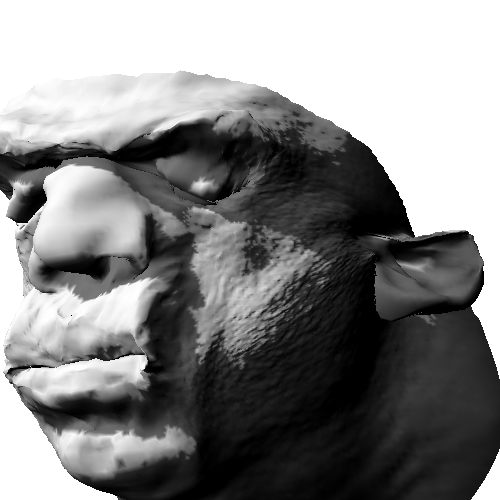
\includegraphics[width=\textwidth]{images/notre-dame}
    \caption{Модель голови схожа на Квазімодо}
    \label{fig:interval:notre-dame}
  \end{subfigure}
  \begin{subfigure}[b]{0.4\textwidth}
    \centering
    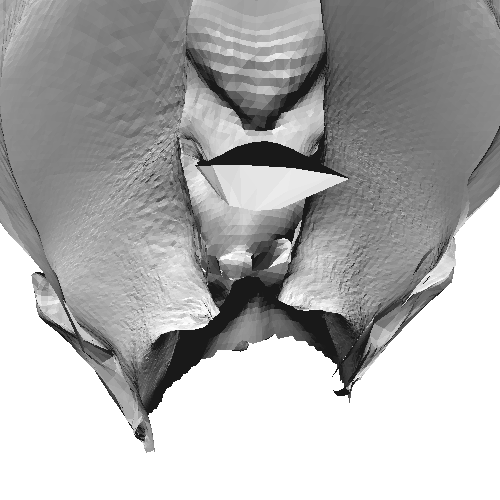
\includegraphics[width=\textwidth]{images/non-human}
    \caption{Модель голови не схожа на голову}
    \label{fig:interval:non-human}
  \end{subfigure}
  \caption{Приклади моделей з завеликими значеннями параметрів}
\end{figure}

\subsection{Різниця параметрів}

У даному підрозділі не будемо враховувати опорні точки,
щоб запобігти завеликих формул.
Проте отриманий результат не втрачає гнучкості
і до нього без проблем можна додати $P_L$.

Ймовірність того,
що дане зображення $t$ було отримано саме з параметрами $x$,
є добутком розглянутих ймовірностей
\begin{equation*}
  \mathbb{P}\left( x, t \right)
  = \mathbb{P}_I\left( t \mcond x \right)
    \cdot \mathbb{P}_X\left( x \right)
  = \delta x^{n + w \cdot h} \cdot \prod_{i \in I}
  \frac{\exp{\left\{ - \frac{\left( t_i - f_i\left( x \right) \right)^2}
       {2 \cdot \sigma_t^2} \right\}}}{\sqrt{2 \cdot \pi \cdot \sigma_t^2}}
  \cdot
  \prod_{i=1}^n
  \frac{\exp{\left\{ - \frac{x_i^2}{2} \right\}}}{\sqrt{2 \cdot \pi}}.
\end{equation*}
Винесемо константи з добутків
\begin{equation*}
  \mathbb{P}\left( x, t \right)
  = \left( \frac{\delta x}{\sqrt{2 \cdot \pi}} \right)^{n + w \cdot h}
    \cdot \prod_{i \in I}
    \frac{\exp{\left\{ - \frac{\left( t_i - f_i\left( x \right) \right)^2}
         {2 \cdot \sigma_t^2} \right\}}}{\sqrt{\sigma_t^2}}
    \cdot
    \prod_{i=1}^n
    \exp{\left\{ - \frac{x_i^2}{2} \right\}}.
\end{equation*}
В даному випадку не можна замінити дисперсію на її оцінку,
бо для кожного $x$ вона буде різною,
через що інтеграл ймовірностей не буде дорівнювати одиниці,
що порушує умову, якій повинна задовольняти ймовірнісна міра
\cite{dorogovtsev:1989}.
Введемо константу
\begin{equation*}
  c_t = \frac{
      \left( 2 \cdot \pi \right)^{- \frac{n + w \cdot h}{2}}
      \cdot \left( \sigma_t^2 \right)^{- \frac{w \cdot h}{2}}
    }{\mathbb{P}\left( t \right)}
\end{equation*}
Ймовірність певного набору параметрів $x$ на даному зображенні $t$
\begin{equation*}
  \mathbb{P}\left( x \mcond t \right)
  = c_t \cdot \delta x^{n + w \cdot h}
    \cdot \exp{\left\{ - \frac{\left\| t - f\left( x \right) \right\|^2}
                              {2 \cdot \sigma_t^2} \right\}}
    \cdot \exp{\left\{ - \frac{\left\| x \right\|^2}{2} \right\}}.
\end{equation*}
Стратегія розпізнавання
\begin{equation*}
  q^*_{\theta}\left( t \right)
  = c_t \cdot \delta x^{n + w \cdot h}
    \cdot \sum_{x \in X}
      x
      \cdot \exp{\left\{ - \frac{\left\| t - f\left( x \right) \right\|^2}
                                {2 \cdot \sigma_t^2} \right\}}
      \cdot \exp{\left\{ - \frac{\left\| x \right\|^2}{2} \right\}}.
\end{equation*}
Щільність розподілу набору параметрів $x$ на даному зображенні $t$
\begin{equation*}
  p\left( x \mcond t \right)
  = c_t
    \cdot \exp{\left\{ - \frac{\left\| t - f\left( x \right) \right\|^2}
                              {2 \cdot \sigma_t^2} \right\}}
    \cdot \exp{\left\{ - \frac{\left\| x \right\|^2}{2} \right\}}.
\end{equation*}
Стратегія розпізнавання у неперервному випадку
\begin{equation*}
  q^*_{\theta}\left( t \right)
  = c_t
    \cdot \int\limits_{x \in X}
      x
      \cdot \exp{\left\{ - \frac{\left\| t - f\left( x \right) \right\|^2}
                                {2 \cdot \sigma_t^2} \right\}}
      \cdot \exp{\left\{ - \frac{\left\| x \right\|^2}{2} \right\}}
    d\,x.
\end{equation*}

\subsection{Попередні результати в контексті Баєсової теорії розпізнавання}

Тепер очевидно,
що у попередніх роботах використовувалася бінарна функція витрат.
Знову розглянему цільову функцію \eqref{eq:energy:face2face}
\begin{equation*}
  E\left( x, \theta \right)
  = \omega_c \cdot \sum_{i \in I' \subset I} \frac{y_i^2}{\left| I' \right|}
  + \omega_r \cdot \sum_{j = 1}^{n} x_j^2
  + \omega_l \cdot \sum_{l \in L} \frac{\Delta_l^2\left( x \right)}
                                       {\left| L \right|}
  \to \min\limits_{x \in X},
\end{equation*}
для якої коефіцієнти $\omega_c$, $\omega_r$ і $\omega_l$
обираються рівними $1$, $2.5 \cdot 10^{-5}$ і $10$ відповідно.
Згідно з \eqref{eq:energy:common} стає зрозуміло,
звідки беруться ваги $\omega$
\begin{equation*}
  \left| I' \right| \cdot
    \sum_{i \in I' \subset I} \frac{y_i^2}{\left| I' \right| \cdot \sigma^2}
  + \left| L \right| \cdot
    \sum_{l \in L} \frac{\Delta_l^2\left( x \right)}
                        {\left| L \right| \cdot \sigma_L^2}
  + \sum_{i = 1}^n x_i^2
  \to \min\limits_{x \in X}.
\end{equation*}
Оскільки $\omega_c = 1$,
а ділення енергії на константу не змінює результату мінімізації,
можна помножити вираз \eqref{eq:energy:common} на дисперсію шуму картинки
та поділити на розмір сегменту, що розглядається
\begin{equation*}
  \sum_{i \in I' \subset I} \frac{y_i^2}{\left| I' \right|}
  + \frac{\sigma^2}{\sigma_L^2} \cdot \frac{\left| L \right|}{\left| I' \right|}
    \cdot \sum_{l \in L} \frac{\Delta_l^2\left( x \right)}{\left| L \right|}
  + \frac{\sigma^2}{\left| I' \right|} \cdot \sum_{i = 1}^n x_i^2
  \to \min\limits_{x \in X}.
\end{equation*}
Маємо систему рівнянь
\begin{equation*}
  \begin{cases}
    \omega_r &= \frac{\sigma^2}{\left| I' \right|}, \\
    \omega_l &= \frac{\sigma^2}{\sigma_L^2}
                \cdot \frac{\left| L \right|}{\left| I' \right|},
  \end{cases}
  \implies
  \begin{cases}
    \sigma^2 &= \omega_r \cdot \left| I' \right|, \\
    \sigma_L^2 &= \frac{\omega_r}{\omega_l} \cdot \left| L \right|.
  \end{cases}
\end{equation*}
Підставимо значення $\omega_r = 2.5 \cdot 10^{-5}$ і $\omega_l = 10$
\begin{equation*}
  \begin{cases}
    \sigma^2 &= 2.5 \cdot 10^{-5} \cdot \left| I' \right|, \\
    \sigma_L^2 &= 2.5 \cdot 10^{-6} \cdot \left| L \right|.
  \end{cases}
\end{equation*}
Бачимо,
що дисперсія шуму лінійно зростає з площею частини зображення,
яку обіймає обличчя.
Для картинки $500 \times 500$ вона дорівнює одиниці,
а для одного мегапікселя це значення вже сягає $25$.
Для більших зображень сама модель голови має замалу точність,
тому немає сенсу розглядати поведінку дисперсії на них.
Дисперсія відхилення опорних точок від дійсного положення
лінійно залежить від їх кількості.
Точних даних немає,
проте використаний для знаходження особливих точок алгоритм
зазвичай демонструється з набором із $194$ опорних точок,
які було запропоновано у базі PUT Face \cite{put-face:2008}.
В такому випадку дисперсія дорівнює $4.85 \cdot 10^{-4}$.
